%To compile as handout, use
%pdflatex "\def\ishandout{1} \input{filename.tex}"
%Defaults to non-handout mode (with slide reveals)
\ifdefined\ishandout
  \documentclass[handout]{beamer}
\else
  \documentclass{beamer}
\fi
 
\usepackage{econ103slides} 

\date{Lecture \# 14}
\begin{document} 

%%%%%%%%%%%%%%%%%%%%%%%%%%%%%%%%%%%%%%%%

\begin{frame}[plain]
	\titlepage 
	

\end{frame} 

%%%%%%%%%%%%%%%%%%%%%%%%%%%%%%%%%%%%%%%%

\begin{frame}
\frametitle{Weighing a Random Sample}
\begin{block}{Bag Contains 100 Candies}
Estimate total weight of candies by weighing a random sample of size 5 and multiplying the result by 20.
\end{block}
\begin{block}{Your Chance to Win}
The bag of candies and a digital scale will make their way around the room \alert{during the lecture}. Each team (2 students) gets a chance to draw 5 candies and weigh them.
\end{block}
\begin{alertblock}{Team with closest estimate wins the bag of candy!}
\end{alertblock}

\end{frame}
%%%%%%%%%%%%%%%%%%%%%%%%%%%%%%%%%%%%%%%%
\begin{frame}
\frametitle{Weighing a Random Sample}
\begin{block}{Procedure}
When the bag and scale reach your team, do the following:
\end{block}
\begin{enumerate}
\item Fold the top of the bag over and shake to randomize.
\item Randomly draw 5 candies \alert{without replacement}.
\item Weigh your sample and record the result \alert{in grams}.
\item Rodrigo will enter your result into his spreadsheet and multiply it by 20 to estimate the weight of the bag.
\item Replace your sample and shake again to re-randomize.
\item Pass bag and scale to next team.
\end{enumerate}
\end{frame}


%%%%%%%%%%%%%%%%%%%%%%%%%%%%%%%%%%%%%%%%


\begin{frame}
\begin{center}
\Huge Sampling Distributions and Estimation -- Part I
\end{center}
\end{frame}


%%%%%%%%%%%%%%%%%%%%%%%%%%%%%%%%%%%%%%%%
\begin{frame}
  \frametitle{Building a Bridge Between Probability and Statistics}
  \begin{block}{Questions to Answer}
  \begin{enumerate}
    \item How accurately do our sample statistics estimate the unknown population parameters?
    \item How can we quantify the uncertainty in our estimates?
  \end{enumerate}
  \end{block}
  \begin{block}{How We'll Proceed}
    \begin{enumerate}
      \item Use sequence of iid RVs as a model for random sampling from a population.
      \item Parameters of these RVs represent population parameters.
      \item Use tools of probability theory to study the behavior of sample statistics. 
    \end{enumerate}
  \end{block}
\end{frame}
%%%%%%%%%%%%%%%%%%%%%%%%%%%%%%%%%%%%%%%%
\begin{frame}
  \frametitle{Step 1: Random Variable as Model for Population}
  \framesubtitle{Treat Population as RV rather than list of objects}
\small
  \begin{tabular}[h]{cc}
    \hline
    \begin{minipage}[t]{0.6\textwidth}
      \begin{block}{Old Way}
       Among 138 million voters, 69 million will vote for Hillary Clinton\\
      \end{block}
    \end{minipage}
    &
    \begin{minipage}[t]{0.4\textwidth}
      \begin{alertblock}{New Way}
       Bernoulli$(p = 1/2)$ RV 
      \end{alertblock}
    \end{minipage} \\
    \hline
    \begin{minipage}[t]{0.6\textwidth}
      \begin{block}{Old Way}
        List of heights for 97 million US adult males with mean 69 in and std.\  dev.\ 6 in \\
      \end{block}
    \end{minipage}
    &
    \begin{minipage}[t]{0.4\textwidth}
      \begin{alertblock}{New Way}
        $N(\mu=69, \sigma^2 = 36)$ RV 
      \end{alertblock}
    \end{minipage} \\
    \hline
  \end{tabular}

  \vspace{1em}
  \alert{In the second example, our model assumes that the distribution of height is symmetric and bell-shaped.}

\end{frame}
%%%%%%%%%%%%%%%%%%%%%%%%%%%%%%%%%%%%%%%%

\begin{frame}
\frametitle{Recall: (Simple) Random Sample}

\begin{block}{Definition in Words}
Select a sample of $n$ objects from a population in such a way that:
	\begin{enumerate}
\item Each member of the population has the same probability of being selected 
\item The fact that one individual is selected does not affect the chance that any other individual is selected
\item Each sample of size $n$ is equally likely to be selected

\end{enumerate}
\end{block}

\begin{alertblock}{Definition in Math}
	$X_1, X_2, \hdots, X_n \sim \mbox{iid } f(x)$ if continuous\\
  $X_1, X_2, \hdots, X_n \sim \mbox{iid } p(x)$ if discrete
\end{alertblock}

\end{frame}

%%%%%%%%%%%%%%%%%%%%%%%%%%%%%%%%%%%%%%%%
\begin{frame}
  \frametitle{Random Sample Means \emph{Sample With Replacement}}


\begin{itemize}
  \item Without replacement $\Rightarrow$ dependence between samples
  \item But sample small relative to popn.\ $\Rightarrow$ dependence negligible.
  \item This means our candy experiment (in progress) isn't bogus.
\end{itemize}
\end{frame}

%%%%%%%%%%%%%%%%%%%%%%%%%%%%%%%%%%%%%%%%
\begin{frame}
  \frametitle{Step 2: iid RVs Represent Random Sampling from Popn.}
  \begin{block}{Who Will Vote for Hillary Clinton Example}
   Poll random sample of 1000 registered voters:
   $$X_1, \hdots, X_{1000} \sim \mbox{ iid Bernoulli}(p = 1/2)$$
  \end{block}
  \begin{block}{Heights of US Males Example}
   Measure the heights of random sample of 50 US males:
   $$Y_1, \hdots, Y_{50}  \sim \mbox{ iid } N(\mu = 69, \sigma^2 = 36)$$
  \end{block}

  \begin{block}{Key Question}
   What do the properties of the population imply about the properties of the sample? 
  \end{block}
\end{frame}
%%%%%%%%%%%%%%%%%%%%%%%%%%%%%%%%%%%%%%%%
\begin{frame}
  \frametitle{What does the population imply about the sample? \hfill
\includegraphics[scale = 0.05]{./images/clicker}}
Suppose that exactly half of US voters plan to vote for Hillary Clinton. 
If you poll a random sample of 4 voters, what is the probability that \emph{none of them} are Hillary supporters?

\pause

\alert{$$(1/2)^4 = 1/16 = 0.0625$$}
\end{frame}
%%%%%%%%%%%%%%%%%%%%%%%%%%%%%%%%%%%%%%%%
\begin{frame}
  \frametitle{What does the population imply about the sample? \hfill
\includegraphics[scale = 0.05]{./images/clicker}}
Suppose that exactly half of US voters plan to vote for Hillary Clinton. 
If you poll a random sample of 4 voters, what is the probability that \emph{exactly half} are Hillary supporters? 

\pause

\alert{$${4 \choose 2} \left( 1/2 \right)^2 \left( 1/2 \right)^2 = 3/8 = 0.375$$}
\end{frame}
%%%%%%%%%%%%%%%%%%%%%%%%%%%%%%%%%%%%%%%%
\begin{frame}
  \frametitle{The rest of the probabilities\dots}
  Suppose that exactly half of US voters plan to vote for Hillary Clinton and we poll a random sample of 4 voters.
  \begin{eqnarray*}
    P\left( \mbox{Exactly 0 Hillary Voters in the Sample} \right) &=& 0.0625\\
    P\left( \mbox{Exactly 1 Hillary Voters in the Sample} \right) &=& 0.25\\
    P\left( \mbox{Exactly 2 Hillary Voters in the Sample} \right) &=& 0.375\\
    P\left( \mbox{Exactly 3 Hillary Voters in the Sample} \right) &=& 0.25\\
    P\left( \mbox{Exactly 4 Hillary Voters in the Sample} \right) &=& 0.0625 
  \end{eqnarray*}

  \vspace{1em}
  \alert{You should be able to work these out yourself. If not, review the lecture slides on the Binomial RV.}
\end{frame}
%%%%%%%%%%%%%%%%%%%%%%%%%%%%%%%%%%%%%%%%
\begin{frame}
  \frametitle{Population Size is Irrelevant Under Random Sampling}
  \framesubtitle{Though we'll see sample size is crucial.}

  \begin{block}{Crucial Point}
    \emph{None} of the preceding calculations involved the population size: I didn't even tell you what it was!
    We'll never talk about population size again in this course.
  \end{block}

  \begin{block}{Why?}
    Since we're drawing with replacement it doesn't matter how many \emph{total voters} there are: all that matters is the \emph{proportion} of Hillary supporters in the population and the number of samples we draw. 
  \end{block}

\end{frame}
%%%%%%%%%%%%%%%%%%%%%%%%%%%%%%%%%%%%%%%%
\begin{frame}
  \frametitle{Step 3: Random Sampling $\Rightarrow$ \emph{Sample Statistics} are RVs} 
  Sample proportions in Hillary election example.
\end{frame}
%%%%%%%%%%%%%%%%%%%%%%%%%%%%%%%%%%%%%%%%
\begin{frame}
  \frametitle{(Sample) Statistic}

  Any function of the data \emph{alone}, e.g.\ sample mean $\bar{x} = \frac{1}{n}\sum_{i=1}^n x_i$. Typically used to estimate an unknown population parameter: e.g.\ $\bar{x}$ is an estimate of $\mu$.

\end{frame}

%%%%%%%%%%%%%%%%%%%%%%%%%%%%%%%%%%%%%%%%
\begin{frame}
\frametitle{Random Sampling}
In other words:
	$$X_1, X_2, \hdots, X_n \sim \mbox{iid } f(x)$$
is a \alert{Random Sample}

	\vspace{1em}
\begin{block}{Statistics}
Sample is drawn randomly, so sample statistics are \emph{also random}. Use what we know about probability theory to analyze the \emph{distribution} of a statistic under random sampling.
\end{block}
\end{frame}

%%%%%%%%%%%%%%%%%%%%%%%%%%%%%%%%%%%%%%%%


\begin{frame}
\frametitle{Estimator versus Estimate}

\begin{block}{Estimator}
An estimator is a function $T(X_1, \hdots, X_n)$ of the random variables we use to represent the random sampling procedure. Hence, it is a random variable itself.
\end{block}
\pause
\begin{block}{Sampling Distribution}
The probability distribution of an Estimator is called a \emph{sampling distribution}.
\end{block}
\pause
\begin{block}{Estimate}
An estimate is a function $T(x_1, \hdots, x_n)$ of the \emph{observed data}, i.e.\ the \emph{realizations} of the random variables we use to represent random sampling. An estimate is a \emph{constant} since the observed data are \emph{constants}
\end{block}

\end{frame}

%%%%%%%%%%%%%%%%%%%%%%%%%%%%%%%%%%%%%%%%


\begin{frame}

\begin{center}
\setlength{\unitlength}{1cm}
\begin{picture}(5,7)
\put(1,6){\framebox(3,1){Population: $f(x)$}}

\put(4.5,6.5){\makebox{\small \alert{\emph{Probability Distribution}}}}
\pause
\put(2.5,6){\vector(0,-1){1}}
\put(0,3){\framebox(5,1){$X_1, X_2, \hdots, X_n \sim \mbox{iid } f(x)$}}
\put(0.5,4.5){\makebox{\small Random Sample of Size $n$}}

\put(-3,3.4){\makebox{\small \alert{\emph{Random Variables}}}}
\pause

\put(0.5,3){\vector(-1,-1){1.5}}
\put(-2.3,0.7){\framebox(2.5,0.65){$x_1^{(1)}, \hdots, x_n^{(1)}$}}
\pause

\put(2,3){\vector(0,-1){1.5}}
\put(0.7,0.7){\framebox(2.5,0.65){$x_1^{(2)}, \hdots, x_n^{(2)}$}}

\pause

\put(3.5,2){\makebox{...}}

\pause

\put(4.5,3){\vector(1,-1){1.5}}
\put(4.8,0.7){\framebox(2.5,0.65){$x_1^{(M)}, \hdots, x_n^{(M)}$}}

\put(-1,-0.2){\makebox{\small $M$ Replications, each containing $n$ Observations}}

\put(5.6,2.6){\makebox{\small \alert{\emph{Realizations}}}}
\put(5.6,2.2){\makebox{\small \alert{\emph{(Constants)}}}}

\end{picture}
\end{center}


\end{frame}
%%%%%%%%%%%%%%%%%%%%%%%%%%%%%%%%%%%%%%%%

\begin{frame}

\begin{center}
\setlength{\unitlength}{1cm}
\begin{picture}(5,7)
\put(-1,5){\framebox(4.5,0.6){$X_1, X_2, \hdots, X_n \sim \mbox{iid } f(x)$}}
\put(-0.7,6){\makebox{\small Random Sample of Size $n$}}


\put(-2.7,5.6){\makebox{\small \alert{\emph{Random}}}}
\put(-2.7,5.2){\makebox{\small \alert{\emph{Variables}}}}

\pause

\put(3.8,5.3){\vector(1,0){1}}
\put(5.5,6){\makebox{\small Estimator}}
\put(5,5){\framebox(2.5,0.6){$T(X_1,\hdots, X_n)$}}



\put(5,4){\makebox{\small \alert{$\displaystyle\bar{X}_n= \frac{1}{n} \sum_{i=1}^n X_i$}}}




\pause

\put(1.2,4.7){\vector(0,-1){2.3}}
\put(-0.2,1.7){\makebox{\small Observations (Data)}}
\put(0,0.7){\framebox(2.5,0.6){$x_1, \hdots, x_n$}}
\put(-2.7,0.9){\makebox{\small \alert{\emph{Constants}}}}

\pause

\put(4.5,1.7){\makebox{\small Estimate}}
\put(4,0.7){\framebox(2.5,0.6){$T(x_1, \hdots, x_n)$}}
\put(2.8,1){\vector(1,0){1}}
\put(4,-0.2){\makebox{\small \alert{$\displaystyle\bar{x}= \frac{1}{n} \sum_{i=1}^n x_i$}}}

\end{picture}
\end{center}


\end{frame}
%%%%%%%%%%%%%%%%%%%%%%%%%%%%%%%%%%%%%%%%



\begin{frame}
\frametitle{Population: All Students in the Class}
\begin{center}
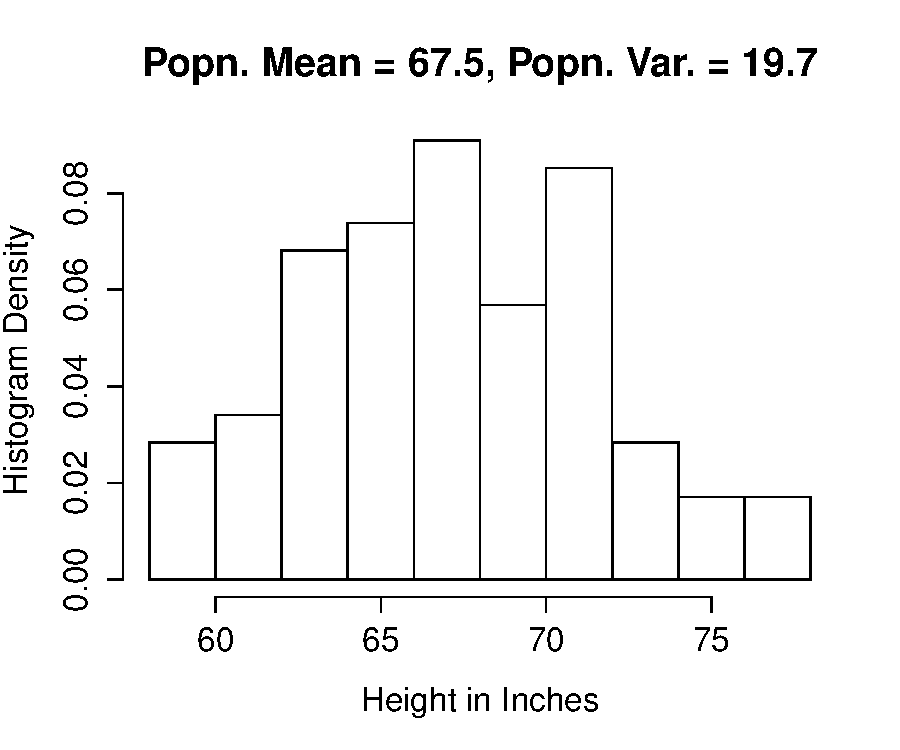
\includegraphics[scale = 0.54]{./images/height_hist}
\end{center}
\end{frame}
%%%%%%%%%%%%%%%%%%%%%%%%%%%%%%%%%%%%%%%%


\begin{frame}

\begin{center}
\setlength{\unitlength}{1cm}
\begin{picture}(5,7)
\put(0,5){\framebox(5,1){$X_1, X_2, \hdots, X_n \sim \mbox{iid } f(x)$}}
\put(0.5,6.5){\makebox{\small Random Sample of Size $n$}}

\pause

\put(0.5,5){\vector(-1,-1){1.5}}
\put(-2.3,2.7){\framebox(2.5,0.65){$x_1^{(1)}, \hdots, x_n^{(1)}$}}

\pause

\put(-1,2.5){\vector(0,-1){1}}
\put(-1.1,0.9){\makebox{\small $\bar{x}_1$}}

\pause

\put(2,5){\vector(0,-1){1.5}}
\put(0.7,2.7){\framebox(2.5,0.65){$x_1^{(2)}, \hdots, x_n^{(2)}$}}

\pause

\put(2,2.5){\vector(0,-1){1}}
\put(1.9,0.9){\makebox{\small $\bar{x}_2$}}

\pause

\put(3.8,3){\makebox{...}}
\put(3.8,1){\makebox{...}}

\pause

\put(4.5,5){\vector(1,-1){1.5}}
\put(4.8,2.7){\framebox(2.5,0.65){$x_1^{(M)}, \hdots, x_n^{(M)}$}}

\pause

\put(6,2.5){\vector(0,-1){1}}
\put(5.9,0.9){\makebox{\small $\bar{x}_M$}}

\pause

\put(-0.5,0){\makebox{\small $M$ Replications yield $M$ \emph{different estimates}}}

\pause

\put(-0.5,-0.6){\makebox{\small \alert{Sampling Distribution: Infinite Replications}}}

\end{picture}
\end{center}


\end{frame}
%%%%%%%%%%%%%%%%%%%%%%%%%%%%%%%%%%%%%%%%
\begin{frame}
\frametitle{Procedure versus Result of the Procedure}
\begin{block}{Procedure = Random Variable}
\begin{itemize}
\item $X_1, \hdots, X_n$ represents \alert{procedure of taking a random sample}. 
\item $\bar{X}_n = \frac{1}{n}\sum_{i=1}^n X_i$ represents \alert{procedure of taking sample mean}  
\end{itemize}
\end{block}
\pause
\begin{block}{Sampling Dist.\ = Probabilistic Behavior of Procedure}
If I repeat the procedure of taking the mean of a random sample over and over for many samples, what relative frequencies do I get \alert{for the sample means?}
\end{block}

\pause
\begin{block}{Result of Procedure = Constant}
 \begin{itemize}
\item $x_1, \hdots, x_n$ is the  \alert{result of sampling}, the observed data. 
\item $\bar{x} = \frac{1}{n}\sum_{i=1}^n x_i$ is the \alert{result of taking sample mean}  
\end{itemize}
\end{block}


\end{frame}
%%%%%%%%%%%%%%%%%%%%%%%%%%%%%%%%%%%%%%%%
\begin{frame}
\frametitle{Procedure? Long-Run Relative Freqencies?}

Why would I advise you not to play the lottery?
\pause
	\begin{itemize}
		\item You may sometimes win, but if you play the lottery many times, on average you will lose money. \pause
		\item Let $X$ be a random variable representing lottery winnings. I am arguing that $E[X]$ - Cost of Ticket $< 0$
	\end{itemize}
\pause
\begin{block}{Procedure = Random Variable}
Making a habit of playing the lottery. Expectation is negative.
\end{block}
\pause
\begin{block}{Result of that Procedure = Constant}
How much you win in a \emph{particular} lottery. Could be greater than or less than cost of ticket in any \emph{individual} instance.
\end{block}
\end{frame}




%%%%%%%%%%%%%%%%%%%%%%%%%%%%%%%%%%%%%%%%
\begin{frame}
\frametitle{Sampling Distribution of $\bar{X}_n = \frac{1}{n}\sum_{i=1}^n X_i$}

\begin{center}
\setlength{\unitlength}{1cm}
\begin{picture}(5,7)
\put(-2,6){\framebox(9,1){Choose $n$ Students from Class List with Replacement}}

\pause

\put(0.5,6){\vector(-1,-1){1.5}}
\put(-2.3,3.7){\framebox(2.5,0.65){Sample 1}}

\pause

\put(-1,3.5){\vector(0,-1){1}}
\put(-1.1,1.9){\makebox{\small $\bar{x}_1$}}

\pause

\put(2,6){\vector(0,-1){1.5}}
\put(0.7,3.7){\framebox(2.5,0.65){Sample 2}}

\pause

\put(2,3.5){\vector(0,-1){1}}
\put(1.9,1.9){\makebox{\small $\bar{x}_2$}}

\pause

\put(3.8,4){\makebox{...}}
\put(3.8,2){\makebox{...}}

\pause

\put(4.5,6){\vector(1,-1){1.5}}
\put(4.8,3.7){\framebox(2.5,0.65){Sample M}}

\pause

\put(6,3.5){\vector(0,-1){1}}
\put(5.9,1.9){\makebox{\small $\bar{x}_M$}}

\pause

\put(-1,1){\makebox{\small Repeat $M$ times $\rightarrow$  get $M$ different sample means}}

\pause

\put(-1.1,0.4){\makebox{\small \alert{Sampling Dist: long run relative frequencies of the $\bar{x}_i$}}}

\end{picture}
\end{center}


\end{frame}
%%%%%%%%%%%%%%%%%%%%%%%%%%%%%%%%%%%%%%%%

\begin{frame}
\frametitle{Height of Econ 103 Students}
\begin{figure}
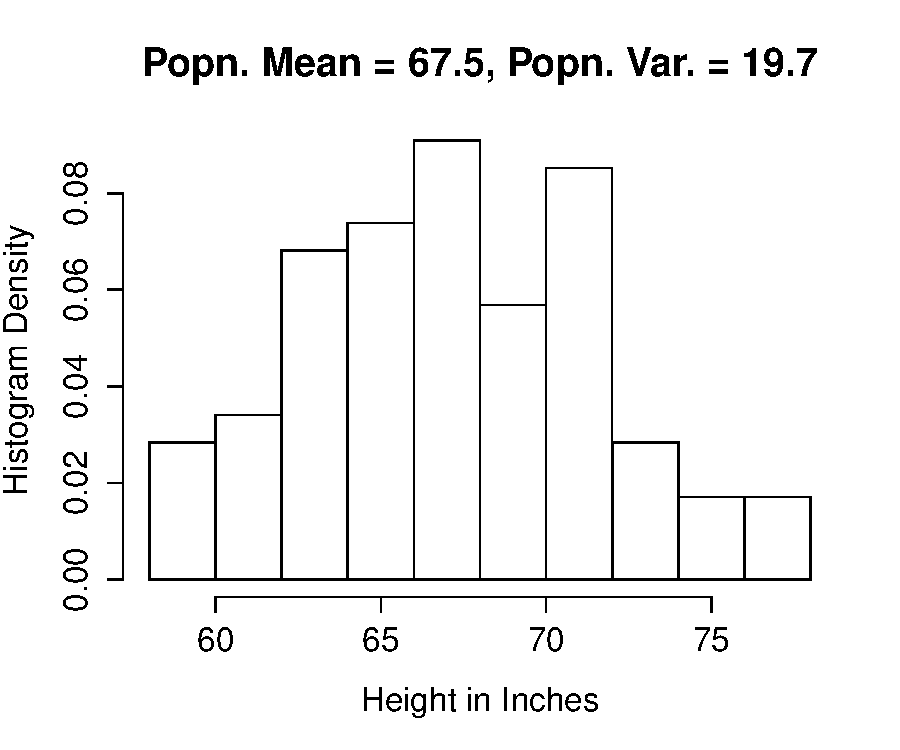
\includegraphics[scale = 0.4]{./images/height_hist}
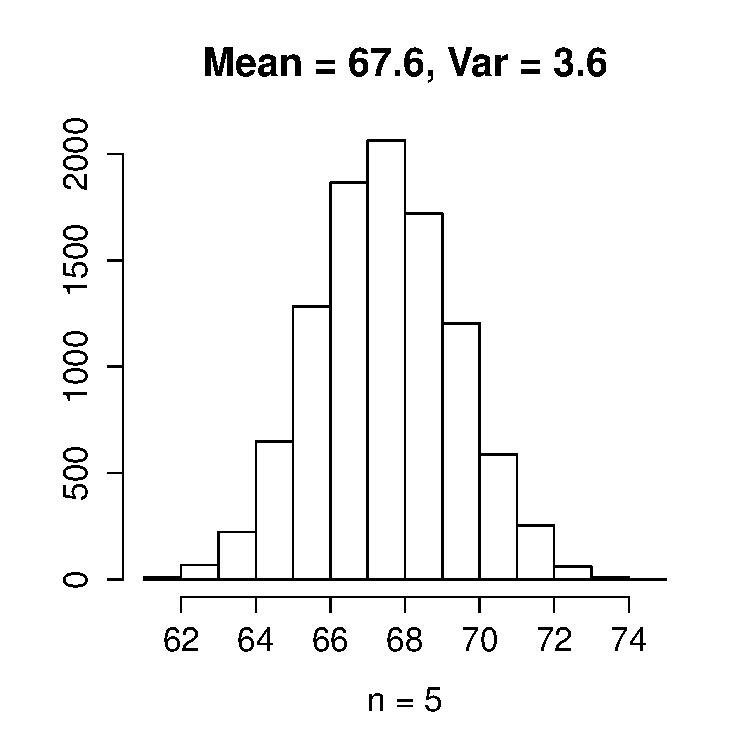
\includegraphics[scale = 0.4]{./images/height_mean_n_5}
\caption{Left: Population, Right: Sampling distribution of $\bar{X}_5$}
\end{figure}
\end{frame}

\begin{frame}
\frametitle{Histograms of sampling distribution of sample mean $\bar{X}_n$}
\alert{Random Sampling With Replacement, 10000 Reps. Each}
\begin{center}
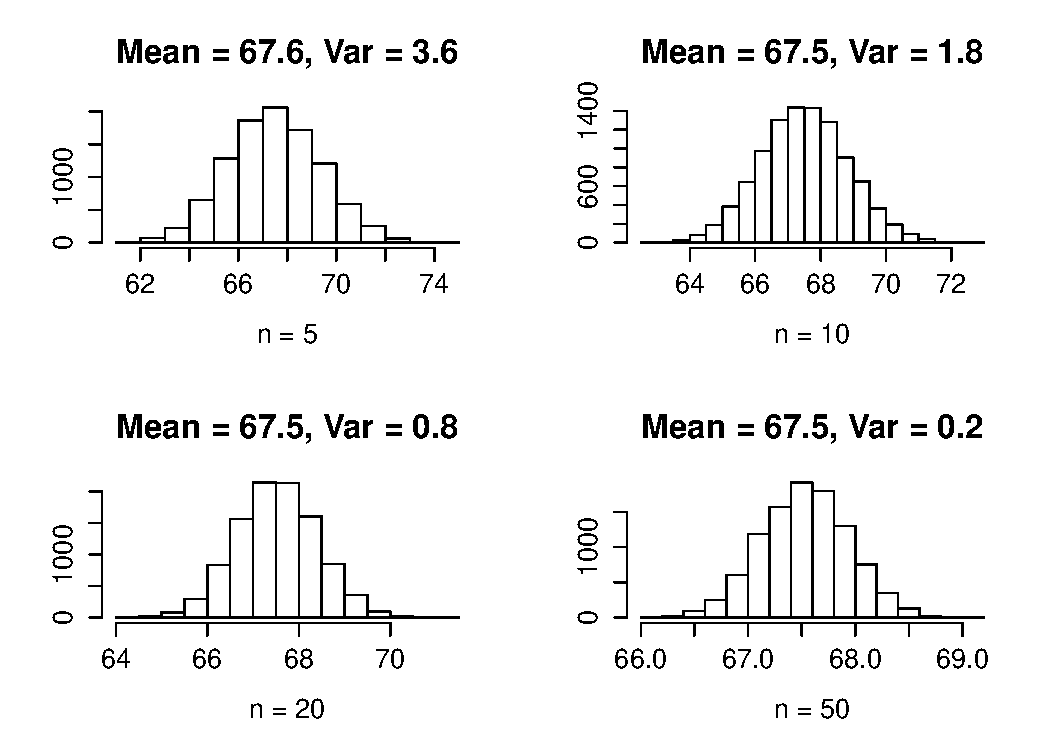
\includegraphics[scale = 0.55]{./images/height_samples}
\end{center}
\end{frame}
%%%%%%%%%%%%%%%%%%%%%%%%%%%%%%%%%%%%%%%%
\begin{frame}
\frametitle{Population Distribution vs.\ Sampling Distribution of $\bar{X}_n$}

\begin{columns} 
\begin{column}[c]{6cm} 

 %FIRST COLUMN HERE 
\begin{figure}
\centering
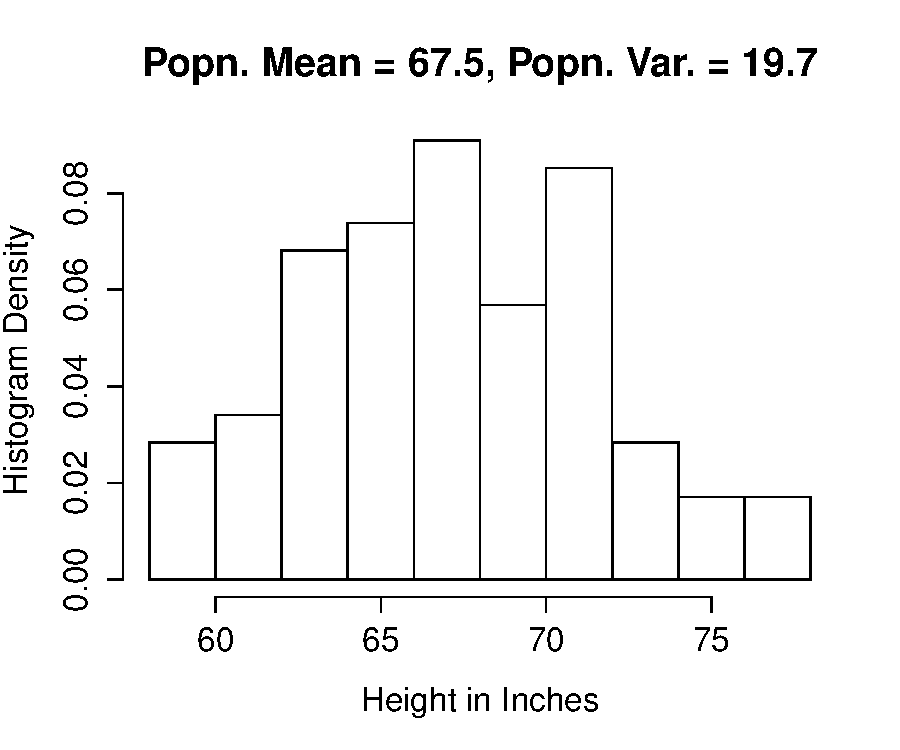
\includegraphics[scale = 0.35]{./images/height_hist}
\end{figure}
\end{column} 
\begin{column}[c]{6cm} 

 %SECOND COLUMN HERE 
 \small
\begin{table}
\begin{tabular}{|rrr|}
\hline
&\multicolumn{2}{c|}{Sampling Dist.\ of $\bar{X}_n$}\\
$n$&Mean&Variance\\
\hline
5&67.6&3.6\\
10&67.5&1.8\\
20&67.5&0.8\\
50&67.5&0.2\\
\hline
\end{tabular}
\end{table}

\end{column} 
\end{columns} 
\begin{alertblock}{Two Things to Notice:}
\begin{enumerate}
	\item Sampling dist.\ ``correct on average'' 
	\item Sampling variability decreases with $n$
\end{enumerate}
\end{alertblock}
\end{frame}

%%%%%%%%%%%%%%%%%%%%%%%%%%%%%%%%%%%%%%%%
\begin{frame}
\frametitle{$X_1,\hdots, X_{9} \sim \mbox{ iid }$ with $\mu=5$, $\sigma^2 =36$. \hfill
\includegraphics[scale = 0.05]{./images/clicker}}

\large Calculate:
	 $$E(\bar{X}) = E\left[\frac{1}{9}(X_1 + X_2 + \hdots + X_{9})\right]$$
\end{frame}
%%%%%%%%%%%%%%%%%%%%%%%%%%%%%%%%%%%%%%%%
\begin{frame}
\frametitle{Mean of Sampling Distribution of $\bar{X}_n$}
\alert{$X_1, \hdots, X_n \sim \mbox{iid with mean }\mu$}
\begin{eqnarray*}
E[\bar{X_n}] = E\left[ \frac{1}{n}\sum_{i=1}^n X_i \right]\pause = \frac{1}{n} \sum_{i=1}^n E[X_i] = \pause\frac{1}{n} \sum_{i=1}^n \mu = \pause \frac{n\mu}{n} =\pause \mu
\end{eqnarray*}
\pause \alert{Hence, sample mean is ``correct on average.'' The formal term for this is \emph{unbiased}.}
\end{frame}

%%%%%%%%%%%%%%%%%%%%%%%%%%%%%%%%%%%%%%%%
\begin{frame}
\frametitle{$X_1,\hdots, X_{9} \sim \mbox{ iid }$ with $\mu=5$, $\sigma^2 = 36$. \hfill
\includegraphics[scale = 0.05]{./images/clicker}}

\large Calculate:
	 $$Var(\bar{X}) = Var\left[\frac{1}{9}(X_1 + X_2 + \hdots + X_{9})\right]$$
\end{frame}
%%%%%%%%%%%%%%%%%%%%%%%%%%%%%%%%%%%%%%%%

\begin{frame}
\frametitle{Variance of Sampling Distribution of $\bar{X}_n$}
\alert{$X_1, \hdots, X_n \sim \mbox{iid with mean }\mu \mbox{ and variance } \sigma^2$}
\begin{eqnarray*}
Var[\bar{X_n}] &=& Var\left[ \frac{1}{n}\sum_{i=1}^n X_i \right] \pause= \frac{1}{n^2} \sum_{i=1}^n Var(X_i) \\
&=& \pause \frac{1}{n^2} \sum_{i=1}^n \sigma^2 = \pause \frac{n\sigma^2}{n^2} = \pause \frac{\sigma^2}{n}
\end{eqnarray*}
\pause
\alert{Hence the variance of the sample mean \emph{decreases linearly with sample size}.}
\end{frame}
%%%%%%%%%%%%%%%%%%%%%%%%%%%%%%%%%%%%%%%%
\begin{frame}
\frametitle{$X_1,\hdots, X_{9} \sim \mbox{ iid }$ with $\mu=5$, $\sigma^2 = 36$. \hfill
\includegraphics[scale = 0.05]{./images/clicker}}

\large Calculate:
	 $$SD(\bar{X}) = SD\left[\frac{1}{9}(X_1 + X_2 + \hdots + X_{9})\right]$$
\end{frame}
%%%%%%%%%%%%%%%%%%%%%%%%%%%%%%%%%%%%%%%%
\begin{frame}
\frametitle{Standard Error}
Std. Dev.\ of estimator's sampling dist.\ is called \alert{standard error}.
\begin{block}{Standard Error of the Sample Mean}
$SE(\bar{X}_n)= \sqrt{Var\left(\bar{X}_n\right)}= \sqrt{\sigma^2/n}=\sigma/\sqrt{n}$
\end{block}
\end{frame}

% \begin{frame}
% \frametitle{Unbiased means ``Right on Average''}

% \begin{block}{Bias of an Estimator}
% Let $\widehat{\theta}_n$ be a sample estimator of a population parameter $\theta_0$. The \emph{bias} of $\widehat{\theta}_n$ is $E[\widehat{\theta}_n] - \theta_0$.
% \end{block}

% \begin{block}{Unbiased Estimator}
% A sample estimator $\widehat{\theta}_n$ of a population parameter $\theta_0$ is called \emph{unbiased} if $E[\widehat{\theta}_n]= \theta_0$
% \end{block}

% \end{frame}


%%%%%%%%%%%%%%%%%%%%%%%%%%%%%%%%%%%%%%%%


\end{document}
